\documentclass[11pt]{article}
\usepackage[portuguese]{babel}
\usepackage{macros}
\usepackage{fancyvrb}
\geometry{a4paper, left=2cm, right=2cm, top=2cm, bottom=1.5cm}
\usepackage{setspace}\onehalfspacing
\usepackage[backend=biber, style=numeric, sorting=none]{biblatex}\addbibresource{referencias_t1.bib}

\begin{document}

\nocite{*}

\begin{center}
    \large Universidade Federal do Rio Grande do Sul \\
    \large Instituto de Matemática e Estatística \\
    \vspace{4cm}
    \huge Simulação Numérica de um Circuito RC \\
    \vspace{1cm}
    \Large Cálculo Numérico II (MAT-01125)  \\
    \vspace{4cm}

    \large\begin{tabular}{rl}
        Aluno: & Leonardo Kawai Suarez - 578511 \\
        Professor: & Dra. Cibele Ladeia Aparecida \\
    \end{tabular}

    \vfill
    \large Porto Alegre, RS \\
    \large \today
\end{center}

\newpage
\tableofcontents

\section{Resumo}

Neste trabalho, implementamos os métodos numéricos de Euler, Heun e Runge-Kutta de ordem 4 para resolver o problema de valor inicial (PVI) associado ao carregamento de um capacitor em um circuito RC. Analisamos a convergência dos métodos para a solução exata do PVI, bem como a dependência do erro em função do passo \(h\). Os resultados confirmaram as ordens de convergência teóricas dos métodos, com RK4 apresentando o menor erro para os passos analisados.

\section{Introdução}

Considera um capacitor, inicialmente descarregado e ligado a uma bateria de fem \(\mathcal{E}\), e seja \(R\) a resistência do circuito. Quando o circuito é fechado, cargas positivas começam a se acumular em uma das placas do capacitor, enquanto cargas negativas se acumulam na outra placa. A tensão \(V\) no capacitor aumenta à medida que ele carrega, e a corrente \(I\) no circuito diminui. Da 1ª lei de Kirchhoff (lei das malhas), sabe-se que a soma das quedas de tensão em um circuito fechado é igual à fem total fornecida pela fonte. Assim, temos a seguinte equação para o circuito RC:

\begin{equation}
    RI(t) - \mathcal{E} + V(t) = 0,
\end{equation} onde \(I(t)\) é a corrente no circuito. Além disso, a corrente \(I\) é relacionada à taxa de variação da tensão \(V\) no capacitor por \(I(t) = C \frac{dV}{dt}\), onde \(C\) é a capacitância do capacitor. Substituindo essa relação na equação de Kirchhoff, obtemos a seguinte equação diferencial ordinária (EDO) para o circuito RC:

\begin{equation}
    RC \frac{dV}{dt} + V = \mathcal{E}.
\end{equation} Essa EDO descreve a evolução da tensão \(V\) no capacitor ao longo do tempo. A constante de tempo do circuito RC é dada por \(\tau = RC\), e ela determina a rapidez com que o capacitor carrega ou descarrega. A solução analítica dessa EDO é dada por

\begin{equation}
    V(t) = \mathcal{E} \left(1 - e^{-\frac{t}{\tau}}\right),
\end{equation} onde \(V(0) = 0\) é a condição inicial para um capacitor inicialmente descarregado. Essa solução mostra que a tensão \(V\) no capacitor aumenta exponencialmente em direção à fem \(\mathcal{E}\) da fonte, com uma taxa de crescimento determinada pela constante de tempo \(\tau\).

\begin{figure}[h]
    \centering
    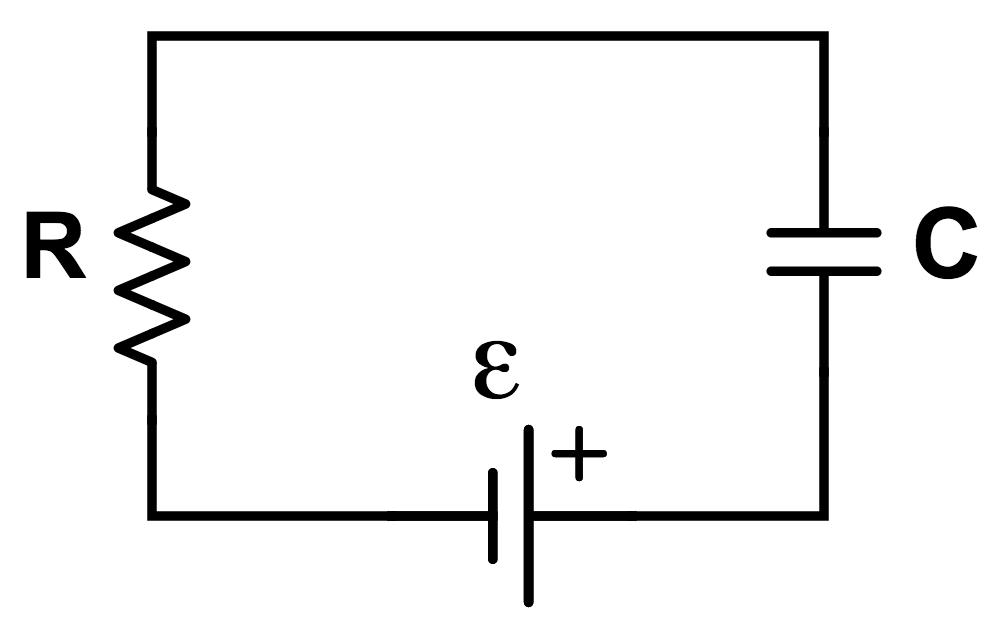
\includegraphics[width=0.5\textwidth]{circuito_rc.png}
    \caption{Circuito RC simples.}
    \label{fig:circuito_rc}
\end{figure}

Resolvemos então o seguinte problema de valor inicial (PVI) para o circuito RC.

\begin{unprblm}[Circuito RC]
    Um capacitor é carregado em um circuito com fonte de \qty{10}{\volt}. A variação da tensão depende da diferença entre a tensão da fonte e a tensão no capacitor, com constante \qty{0.5}{\per\second}. Assim, temos o seguinte problema de valor inicial

    \begin{equation}
        \frac{dV}{dt} = 0.5 (10 - V), \quad V(0) = 0,
    \end{equation} onde \(V\) é a tensão (\unit{\volt}) e \num{0.5} é a constante do circuito. Resolva o PVI com os métodos de Euler e Runge-Kutta (ordens \numlist{2;4}) no intervalo \(0 \leq t \leq t_{\max} = \qty{10}{\second}\) com passos \(h = \qtylist{1;0.2;0.05}{\second}\). Depois, compare os resultados com a solução analítica, dada por

    \begin{equation}
        V(t) = 10 (1 - e^{-0.5t}).
    \end{equation}
\end{unprblm}

\section{Metodologia}

Implementamos os métodos de Euler, Heun e RK4 em Python para resolver o PVI do circuito RC com os programas listados a seguir. O algoritmo \cref{lst:metodos_edo} implementa os métodos numéricos para resolver EDOs, enquanto o algoritmo \cref{lst:resolucao_edo} aplica esses métodos para resolver o PVI do circuito RC, comparar os resultados com a solução analítica e analisar os erros.

\begin{lstlisting}[style=python-custom, caption={Algoritmos para os métodos de Euler, Heun e RK4.}, label={lst:metodos_edo}]
    import numpy as np

    def euler(f, u0, t0, tf, h):
        """
        euler's method to approximate solution u(t) of an ordinary differential equation du/dt = f(t, u)

        input:
            f: derivative of u(t) wrt time
            u0: initial condition
            t0: start of time interval
            tf: end of time interval
            h: step size
        output:
            t: ndarray (tf-t0)/h
            u: ndarray (u(t_n))
        """
        n = int((tf-t0)/h)
        t = np.linspace(t0, tf, n+1) # create time vector with n+1 elements (or n subintervals)
        u = np.zeros(len(t)) # start solution vector
        u[0] = u0 # set initial condition

        for k in range(0, len(t) - 1):
            u[k+1] = u[k] + h * f(t[k], u[k])
        return t, u

    def heun(f, u0, t0, tf, h):
        """
        improved euler's method (or Heun's method) to approximate solution u(t) of an ordinary differential equation du/dt = f(t, u)

        input:
            f: derivative of u(t) wrt time
            u0: initial condition
            t0: start of time interval
            tf: end of time interval
            h: step size
        output:
            t: ndarray (tf-t0)/h
            u: ndarray (u(t_n))
        """
        n = int((tf-t0)/h)
        t = np.linspace(t0, tf, n+1) # create time vector with n+1 elements (or n subintervals)
        u = np.zeros(len(t)) # start solution vector
        u[0] = u0 # set initial condition

        for k in range(0, len(t) - 1):
            k1 = f(t[k], u[k])
            k2 = f(t[k+1], u[k] + h * k1)
            u[k+1] = u[k] + (h/2) * (k1 + k2)
        return t, u

    def rk4(f, u0, t0, tf, h):
        """
        classic Runge-Kutta method to approximate solution u(t) of an ordinary differential equation du/dt = f(t, u)

        input:
            f: derivative of u(t) wrt time
            u0: initial condition
            t0: start of time interval
            tf: end of time interval
            h: step size
        output:
            t: ndarray (tf-t0)/h
            u: ndarray (u(t_n))
        """
        n = int((tf-t0)/h)
        t = np.linspace(t0, tf, n+1) # create time vector with n+1 elements (or n subintervals)
        u = np.zeros(len(t)) # start solution vector
        u[0] = u0 # set initial condition

        for k in range(0, len(t) - 1):
            k1 = f(t[k], u[k])
            k2 = f(t[k] + h/2, u[k] + (h/2) * k1)
            k3 = f(t[k] + h/2, u[k] + (h/2) * k2)
            k4 = f(t[k+1], u[k] + h * k3)
            u[k+1] = u[k] + (h/6) * (k1 + 2 * k2 + 2 * k3 + k4)
        return t, u
\end{lstlisting}

\begin{lstlisting}[style=python-custom, caption={Resolução do PVI do circuito RC usando os métodos de Euler, Heun e RK4.}, label={lst:resolucao_edo}]
    import numpy as np
    import matplotlib.pyplot as plt
    from tabulate import tabulate
    from exercicios_py.metodos_edo import euler, heun, rk4

    #------------------------------------------
    # define o problema de valor inicial
    #------------------------------------------
    def f(t, v):
        return 0.5 * (10 - v)
    v0, t0, tf = 0, 0, 10

    def exata_v(t):
        return 10 * (1 - np.exp(-0.5 * t))

    #------------------------------------------------------
    # imprime tabela com resultados e plota os gráficos
    #------------------------------------------------------
    h_vetor = np.array([1, 0.2, 0.05])
    cores = ['red', 'green', 'blue']

    # cria primeira figura com 3 subplots para comparar os metodos numericos
    fig1, (ax1, ax2, ax3) = plt.subplots(1, 3, sharex=True, sharey=True)
    fig1.suptitle('Comparação dos métodos numéricos')
    fig1.supxlabel(r'$t$ (s)')
    fig1.supylabel(r'$\tilde{V}(t)$ (V)')
    ax1.set_title('Euler')
    ax2.set_title('Heun')
    ax3.set_title('RK4')
    axs = [ax1, ax2, ax3]

    # plota a solucao exata em todos os subplots da figura 1
    t_plot = np.linspace(t0, tf, 100)
    for ax in axs:
        ax.plot(t_plot, exata_v(t_plot), label='exata', color='black', linestyle='--')

    # cria segunda figura para analisar o erro (em escala logaritmica) em funcao do passo h
    fig2, ax4 = plt.subplots()
    ax4.set_title(r'Análise do erro em $t_{max}$ em função do passo $h$')
    ax4.set_xlabel(r'$h$')
    ax4.set_ylabel(r'$\vert V(10)-\tilde{V}(10) \vert$')
    ax4.loglog() 
    ax4.xaxis.set_inverted(True)

    # plota curvas de referencia para O(h), O(h^2) e O(h^4) na figura 2
    href = np.linspace(h_vetor.min(), h_vetor.max(), 100)
    ax4.plot(href, href, label=r'O(h)', color='gray', linestyle='--')
    ax4.plot(href, href**2, label=r'O($h^2$)', color='gray', linestyle=':')
    ax4.plot(href, href**4, label=r'O($h^4$)', color='gray', linestyle='-.')

    # cria lista para armazenar os erros maximos e os erros em tf de cada metodo numerico para imprimir na tabela de dados
    dados = []
    # cria listas para armazenar os erros em tf de cada metodo numerico para plotar na figura 2
    erros_euler = []
    erros_heun = []
    erros_rk4 = []

    for h, cor in zip(h_vetor, cores):
        t_euler, v_euler = euler(f, v0, t0, tf, h) # calcula solucao numerica com metodo de Euler
        t_heun, v_heun = heun(f, v0, t0, tf, h) # calcula solucao numerica com metodo de Heun
        t_rk4, v_rk4 = rk4(f, v0, t0, tf, h) # calcula solucao numerica com metodo de RK4
        
        ax1.plot(t_euler, v_euler, label=f'$h={h}$', color=cor)
        ax2.plot(t_heun, v_heun, label=f'$h={h}$', color=cor)
        ax3.plot(t_rk4, v_rk4, label=f'$h={h}$', color=cor)
        
        # funcao para calcular o erro maximo e o erro em tf de uma solucao numerica em relacao a solucao exata
        def calc_erros(t, v):
            erros = np.fabs(exata_v(t) - v)
            return np.max(erros), erros[-1]

        # calcula os erros maximo e em tf para cada metodo numerico e armazena os resultados na tabela de dados
        e_max, e_tf = calc_erros(t_euler, v_euler)
        erros_euler.append(e_tf)
        dados.append(['Euler', h, e_max, e_tf])
        
        e_max, e_tf = calc_erros(t_heun, v_heun)
        erros_heun.append(e_tf)
        dados.append(['Heun', h, e_max, e_tf])

        e_max, e_tf = calc_erros(t_rk4, v_rk4)
        erros_rk4.append(e_tf)
        dados.append(['RK4', h, e_max, e_tf])

    # plota os erros em tf de cada metodo numerico na figura 2
    ax4.plot(h_vetor, erros_euler, '-o', color='red', label='Euler')
    ax4.plot(h_vetor, erros_heun, '-s', color='green', label='Heun')
    ax4.plot(h_vetor, erros_rk4, '-^', color='blue', label='RK4')

    # configura legendas e grades para os graficos e imprime a tabela de dados
    for ax in axs:
        ax.legend(fontsize='small')
        ax.grid(True, alpha=0.3)
    ax4.legend(fontsize='small'); ax4.grid(True, alpha=0.3)

    print(tabulate(dados, headers=['metodo', 'passo (h)', 'erro maximo', 'erro em T_max'], tablefmt='orgtbl', floatfmt=('g', 'g', '.15e', '.15e')))

    plt.tight_layout()
    fig1.savefig('calculo_numerico/comparacao_metodos.pdf', dpi=300, bbox_inches='tight')
    fig2.savefig('calculo_numerico/analise_erro.pdf', dpi=300, bbox_inches='tight')
    plt.show()
\end{lstlisting}

\section{Resultados e Conclusão}

Apresentamos os resultados de \cref{lst:resolucao_edo} abaixo. A primeira figura mostra a comparação dos métodos numéricos com a solução exata, enquanto a segunda figura apresenta a análise dos erros em função do passo \(h\). A tabela de dados mostra os erros máximos e os erros em \(t_{\max}\) para cada método numérico e passo utilizado. 

\begin{figure}[h]
    \centering
    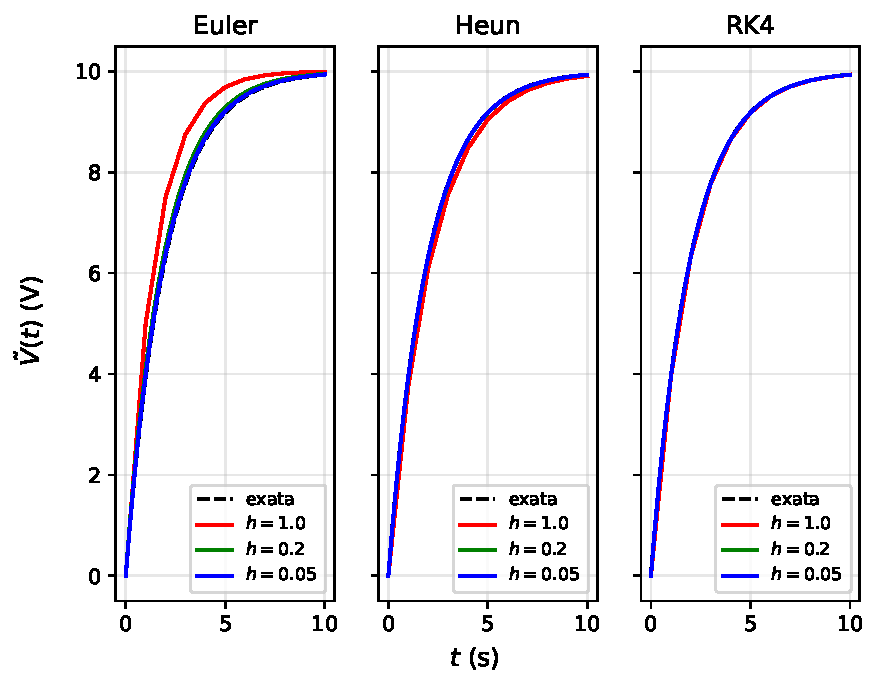
\includegraphics[width=0.9\textwidth]{comparacao_metodos.pdf}
    \caption{Comparação dos métodos numéricos com a solução exata.}
    \label{fig:comparacao_metodos}
\end{figure}

\begin{figure}[H]
    \centering
    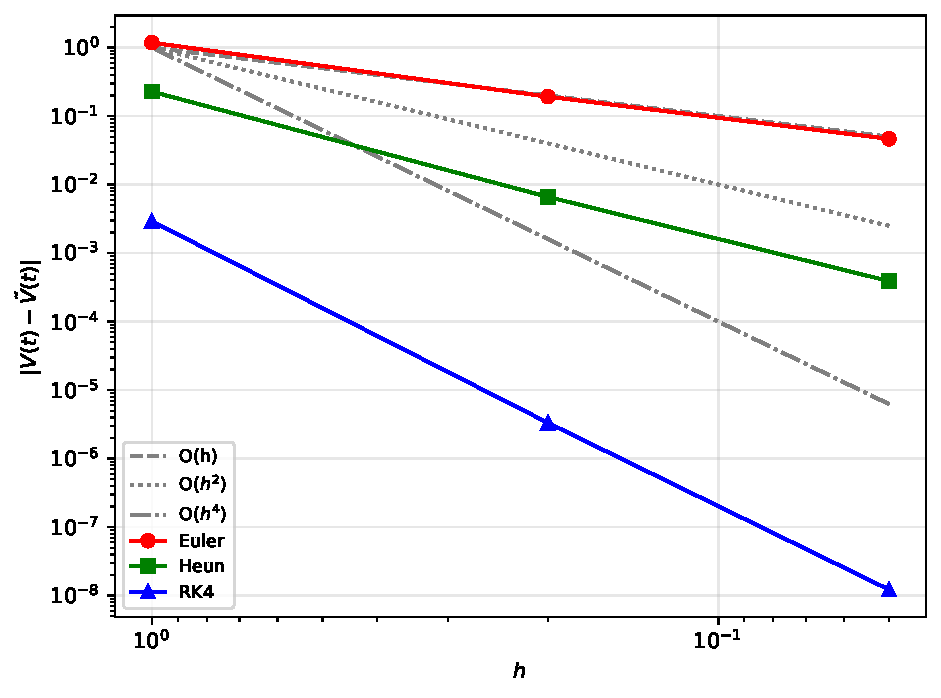
\includegraphics[width=0.9\textwidth]{analise_erro.pdf}
    \caption{Análise dos erros dos métodos numéricos.}
    \label{fig:analise_erro}
\end{figure}

\begin{table}[H]
    \centering
    \caption{Erros máximos e erros em \(t_{\max}\) para cada método numérico e passo utilizado.}
    \label{tab:erros}
    \begin{tabular}{cccc}
        \toprule
        Método & Passo \(h\) & Erro Máximo & Erro em \(t_{\max}\) \\
        \midrule
        Euler & 1 & \(1.178794411714423 \times 10^{-0}\) & \(5.761384499085409 \times 10^{-2}\) \\
        Heun & 1 & \(2.274555882855767 \times 10^{-1}\) & \(2.357000018643873 \times 10^{-2}\) \\
        RK4 & 1 & \(2.914030125855227 \times 10^{-3}\) & \(2.672847229518993 \times 10^{-4}\) \\
        Euler & 0.2 & \(1.920100107144238 \times 10^{-1}\) & \(1.584171791765243 \times 10^{-2}\) \\
        Heun & 0.2 & \(6.615436621094872 \times 10^{-3}\) & \(6.080125442835538 \times 10^{-4}\) \\
        RK4 & 0.2 & \(3.332410560830112 \times 10^{-6}\) & \(3.051766963579894 \times 10^{-7}\) \\
        Euler & 0.05 & \(4.647001283561725 \times 10^{-2}\) & \(4.149476121153128 \times 10^{-3}\) \\
        Heun & 0.05 & \(3.904854541776359 \times 10^{-4}\) & \(3.576754513545666 \times 10^{-5}\) \\
        RK4 & 0.05 & \(1.222741996542709 \times 10^{-8}\) & \(1.119762060852736 \times 10^{-9}\) \\
        \bottomrule
    \end{tabular}
\end{table}

Da \autoref{fig:comparacao_metodos}, verifica-se de imediato a convergência dos métodos numéricos para a solução exata à medida que o passo \(h\) diminui. Como esperado, os métodos de ordem mais alta (Heun e RK4) apresentaram erros significativamente menores do que o método de Euler, especialmente para \(h=\qty{1}{\second}\). Perceba que o erro máximo ocorre próximo ao início do carregamento (regime transiente), onde a curvatura da solução é mais acentuada. Isso é consistente com o erro de truncamento local do método de Euler, por exemplo, que é proporcional à segunda derivada da solução, a qual é maior nos primeiros instantes de tempo. No regime estacionário (próximo a \(t_{\max}\)), a solução se aproxima da fem \(\mathcal{E}\) e a curvatura diminui, o que explica a redução do erro em \(t_{\max}\) para todos os métodos numéricos.

A \autoref{tab:erros} mostra que o método de Euler tem um erro que decresce linearmente com \(h\), enquanto os métodos de Heun e RK4 têm erros que decrescem quadraticamente e quarticamente, respectivamente, confirmando as ordens de convergência teóricas desses métodos. De fato, ao dividir o passo \(h\) por \num{5}, o erro máximo do método de Euler diminuiu \(\frac{1.18 \times 10^{-0}}{1.92 \times 10^{-1}} \approx 6.15\) vezes, o que é consistente com a ordem de convergência \(O(h)\). Já para o método de Heun, o erro máximo diminuiu \(\frac{2.27 \times 10^{-1}}{6.62 \times 10^{-3}} \approx 34.3\) vezes (\(O(h^2)\)). Por fim, para o método de RK4, o erro máximo diminuiu \(\frac{2.91 \times 10^{-3}}{3.33 \times 10^{-6}} \approx 874\) vezes, de acordo com a ordem \(O(h^4)\).

Ainda, observa que o método de RK4 com passo \(h=1\) apresentou erro menor do que o método de Euler com passo \(h=0.05\). Isso porque o método de RK4 envolve computar quatro avaliações da função \(f\) por passo, o que permite uma aproximação muito mais precisa de \(V'(t)\) e, consequentemente, uma solução numérica mais próxima da solução exata, mesmo com um passo maior. Em contraste, o método de Euler, sendo um método de primeira ordem, tem uma aproximação mais grosseira de \(V'(t)\) e, portanto, requer passos menores para alcançar a mesma precisão.

A ordem de convergência dos métodos pode ser facilmente visualizada na \autoref{fig:analise_erro}, onde as curvas de referência para \(O(h)\), \(O(h^2)\) e \(O(h^4)\) mostram claramente a taxa de decrescimento dos erros para cada método numérico. Usando escala logarítmica, é possível observar o paralelismo entre as curvas dos erros e as curvas de referência, confirmando as ordens de convergência teóricas dos métodos de Euler, Heun e RK4.

\printbibliography


\end{document}